\chapter{Proof-of-concept implementáció}\label{ch:proof-of-concept-implementáció}

A proof-of-concept implementáció célja két — egy termelő és egy fogyasztó fél között felépíteni egy WebRTC datachannel-t
dedikált signaling szolgáltatás nélkül.
Az implementáció két, Node.JS környezetben futó JavaScript alkalmazás.
A DHT-t a bittorrent-dht nyílt forráskódú könyvtár implementálja.
Indítás előtt két Ed25519 kulcspárt szükséges generálni:

\begin{lstlisting}[label={lst:lstlisting3}]
const ed = require("bittorrent-dht-sodium");

const keyPair = ed.keygen();
console.log({
    pk: keyPair.pk.toString("hex"),
    sk: keyPair.sk.toString("hex"),
});
\end{lstlisting}

A termelő fél létrehoz egy RTCPeerConnection példányt, majd miután létrejött a WebRTC kapcsolat, létrehoz egy datachannel-t,
és ezen másodpercenként dátummal ellátott teszt üzenetet küld.

\begin{lstlisting}[label={lst:lstlisting4}]
async function main() {
    const connection = new RTCPeerConnection();
    const signaling = new Signaling(keyPair, password, cacheInvalidation);
    signaling.startListening();

    connection.onicecandidate = (event) => {
        if (event.candidate) {
            log("sent ice candidate");
            signaling.sendICECandidate(event.candidate);
        }
    };

    signaling.on("icecandidate", (candidate) => {
        log("got ice candidate");
        connection.addIceCandidate(new RTCIceCandidate(candidate));
    });

    const channel = connection.createDataChannel();

    const offer = await connection.createOffer();
    connection.setLocalDescription(offer);

    signaling.on("offer", (answer) => {
        log("got answer");
        connection.setRemoteDescription(answer);
    });

    await signaling.sendOffer(offer);
    log("sent offer");

    setInterval(() => {
        if (channel.readyState !== "open") {
            return;
        }

        signaling.stopListening();

        channel.send(`hello there! :) ${new Date().toISOString()}`);
    }, 1000);
}
\end{lstlisting}

A fogyasztó fél figyeli a termelő által létrehozott WebRTC offer jelenlétét, majd ha létrejött a datachannel, az ezen
érkező teszt üzeneteket a folyamat stdout-jára írja ki.
Ennek forráskódja nagy mértékben hasonlít a termelő fél kódjára.
Az üzenetek fogadását a következő részlet mutatja be:

\begin{lstlisting}[label={lst:lstlisting3}]
connection.ondatachannel = ({ channel }) => {
    signaling.stopListening();
    channel.addEventListener("message", (e) => {
        log(e.data);
    });
};
\end{lstlisting}

A DHT alapú signaling részleteit a Signaling nevű osztály absztrahálja.
Konstruktorának három paramétere van:

\begin{lstlisting}[label={lst:lstlisting5}]
const signaling = new Signaling(keyPair, password, cacheBurst);
\end{lstlisting}

Az első paraméter a generált kulcspár, a második a másik fél kulcspárjának publikus része, a harmadik paraméterre pedig
később tér ki a dolgozat.
Az adatok küldése a következőképp van implementálva:

\begin{lstlisting}[label={lst:lstlisting6}]
async _send(bucket, value) {
    const bucketId = `${this.cacheBurst}:${bucket}`;
    const md5BucketId = crypto.createHash("md5").update(bucketId).digest();

    const bufCompressed = await compress(value);
    const message = {
        k: this.keyPair.pk,
        salt: md5BucketId,
        seq: this.seq++,
        v: bufCompressed,
        sign: this.sign.bind(this),
    };

    return new Promise((resolve, reject) => {
        this.dht.put(message, (err, hash) => {
            if (err) {
                reject(err);
                return;
            }

            resolve(hash);
        });
    });
}
\end{lstlisting}

Ahhoz, hogy az implementáció több bucket-be is képes legyen adatot írni, a BEP44 protokoll által definiált salt-ot
használja.
A salt a cacheBurst változó és a bucket név konkatenációjának MD5 hash-je.
A DHT-ban tárolt adat így a függvény value paraméterének tömörített változata a salt-tal ellátva, aláírva a kulcspár publikus
részével.
Az üzenet szekvenciaszáma minden írásnál eggyel nő.
A tömörítés deflate algoritmussal történik.

A DHT-ból történő olvasás az alábbi módon van implementálva:

\begin{lstlisting}[label={lst:lstlisting7}]
async getBucket(bucket) {
    const md5Bucket = crypto.createHash("md5").update(`${this.cacheBurst}:${bucket}`).digest();
    const keyBuffer = this.dht._hash(Buffer.concat([this.password, md5Bucket]));

    const result = await this.queryDHT(keyBuffer.toString("hex"), md5Bucket);

    return decompress(result.v);
}

queryDHT(key, salt) {
    return new Promise((resolve, reject) => {
        const options = {
            verify: ed.verify,
            cache: false,
            salt,
        };
        this.dht.get(key, options, (err, result) => {
            if (err) {
                reject(err);
                return;
            }
            if (!result) {
                reject(new Error("no result"));
                return;
            }
            resolve(result);
        });
    });
}
\end{lstlisting}
A DHT-beli kulcs a másik fél publikus kulcsából és az írásnál látott módon generált salt-ból van származtatva a DHT belső
hash függvényével.
A~\ref{fig:prod} és~\ref{fig:cons} képernyőképek a termelő és a fogyasztó csomópontot mutatják be futás közben.

\begin{figure}[!ht]
    \centering
    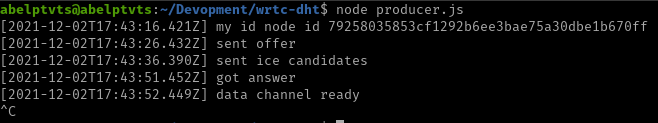
\includegraphics[width=120mm, keepaspectratio]{figures/producer}
    \caption{A termelő futás közben}
    \label{fig:prod}
\end{figure}

\begin{figure}[!ht]
    \centering
    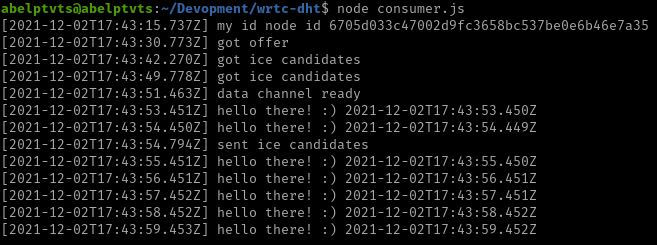
\includegraphics[width=120mm, keepaspectratio]{figures/consumer}
    \caption{A fogyasztó futás közben}
    \label{fig:cons}
\end{figure}


\section{Cache invalidáció}\label{sec:cache-invalidáció}
A DHT-be történő írás során a publikus tracker-ök meghatározatlan ideig tárolják az hozzájuk érkező adatokat.
Emiatt ha a proof-of-concept implementáció újraindul, a csatlakozás nem tud létrejönni, mivel a két fél a folyamatos
lekérdezés során elavult WebRTC offer-eket kap.
Az elvárt működéshez szükséges az, hogy a bucket-ek teljesen üresek legyenek.
Ezt a problémát oldja meg a Signalig osztály cacheBurst paramétere.
A cacheBurst paraméter egy szám, ami minden salt-ban szerepel, így garantálva, hogy az implementáció teljesen új bucket-eket
használ induláskor.
A proof-of-concept implementáció használata során a cacheBurst paramétert \emph{manuálisan} kell állítani.

%TODO possible improvements